\chapter{Anhang}
\thispagestyle{empty}
\section*{Sonnenstandberechnung}\label{Anhang: Sonnenstand}
Die Sonnenstandberechnung (Sonnenhöhe $\gamma_\text{s}$ und Sonnenazimut $\alpha_\text{S}$) ist auf Grundlage des in DIN-5034 \cite{DIN5034} vorgestellten Algorithmus erfolgt. Folgend werden die verwendeten Gleichungen aus \citet{Quaschning2015} dargestellt:

\begin{enumerate}
\item Hilfparameter J' des DIN-Algorithmus:\\
	\begin{equation*}
		J' = 360\text{°} \cdot \dfrac{\text{Tag des Jahres}}{\text{Tage im Jahr}}
	\end{equation*}
\item Sonnendeklination $\delta(J')$ in °
	\begin{equation*}
		\delta(J') = 0,3948 - 23,2559 \cdot \cos(J' - 9,1\text{°}) - 0,3915 \cdot \cos(2J' + 5,4\text{°}) - 0,1764 \cdot \cos(3J'+ 26\text{°})
	\end{equation*}
\item  Zeitgleichung in Minuten
	\begin{equation*}
		Zgl(J') = 0,0066 + 7,3525 \cdot \cos(J' + 85,9\text{°}) + 9,9359 \cdot \cos(2J' + 108,9\text{°}) + 0,3387 \cdot \cos(3J' + 105,2\text{°})
	\end{equation*}
\item Bestimmung der mittleren Ortszeit MOZ in Stunden über die lokale Uhrzeit LZ, die Zeitzone (Stundendifferenz zu UTC-Zeit) und der geographischen Länge $\lambda$
	\begin{equation*}
		\text{MOZ} = \text{LZ} - \text{Zeitzone} + \dfrac{4 \cdot \lambda}{60} 
	\end{equation*}
\item Wahre Ortszeit über Zgl
	\begin{equation*}
		\text{WOZ} = \text{MOZ} - Zgl(J')
	\end{equation*}
\item Stundenwinkel
	\begin{equation*}
		\omega = (12 - \text{WOZ}) \cdot \dfrac{15\text{°}}{\text{h}}
	\end{equation*}
\item[$\Rightarrow$] Sonnenhöhe $\gamma_\text{s}$ über die geographische Breite $\varphi$:
	\begin{equation*}
		\gamma_\text{s} = \arcsin(\cos\omega \cdot \cos\varphi \cdot \cos\delta + \sin\varphi \cdot \sin\delta)
	\end{equation*}
\item[$\Rightarrow$] Sonnenazimut $\alpha_\text{s}$:
	\begin{equation*}
		\alpha_\text{s} = 	\begin{cases}
								180\text{°} - \arccos\dfrac{\sin\gamma_\text{s} \cdot \sin\varphi - \sin\delta}{\cos\gamma_\text{s} \cdot \cos\varphi} & \text{für WOZ $\geq$ 12}\\
								\\
								180\text{°} + \arccos\dfrac{\sin\gamma_\text{s} \cdot \sin\varphi - \sin\delta}{\cos\gamma_\text{s} \cdot \cos\varphi} & \text{für WOZ $<$ 12}
							\end{cases}
	\end{equation*}
\end{enumerate}

\section*{Abbildungen}
	\begin{figure*}[ht]
		\centering
		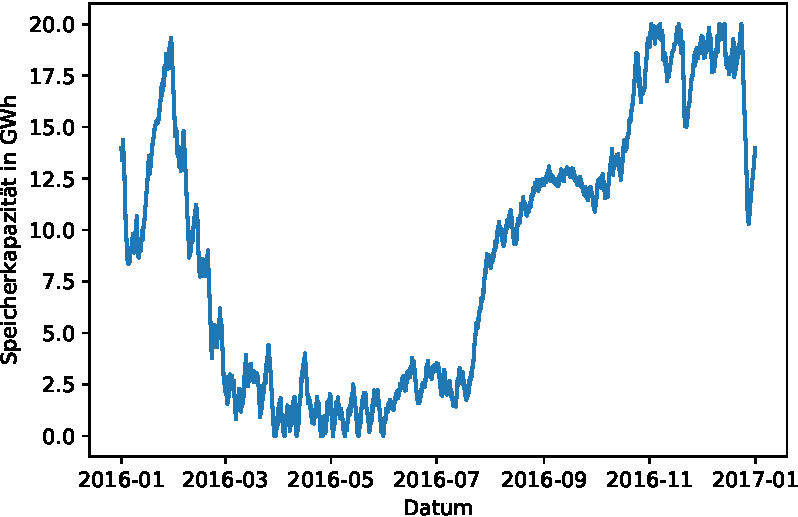
\includegraphics[width=0.8\textwidth]{Speicherverhalten_Photovoltaik-cropped.pdf}
		\captionof{figure}{Darstellung des Ladezustands des saisonalen Wärmespeichers innerhalb des Photovoltaik-Konzepts}
		\label{Anhang: Ladezustand}
	\end{figure*}